\documentclass[12pt]{article}
\usepackage[a4paper, total={7.5in, 11in}]{geometry}
%\usepackage{array}
\usepackage{graphicx, subfig, wrapfig, fancyhdr, lastpage, multicol ,color,arydshln,makecell, mhchem, multirow}
\newcommand\headerMe[2]{\noindent{}#1\hfill#2}
\usepackage[mathscr]{euscript}
\usepackage{tabularray}

\setlength{\columnseprule}{1pt}
\def\columnseprulecolor{\color{blue}}


\pagestyle{fancy}
\fancyhf{}

\cfoot{ \vspace{-0.8cm}\em{Page \thepage \hspace{1pt} / \pageref{LastPage}}}
\begin{document}

\headerMe{Royaume du Maroc}{année scolaire \emph{2023-2024}}\\
\headerMe{Ministère de l'Éducation nationale, }{  Professeur :\emph{Zakaria Haouzan}}\\
\headerMe{du Préscolaire et des Sports}{Établissement : \emph{Lycée SKHOR qualifiant}}\\
%\vspace{-1cm}
\begin{center}
Devoir Surveillé  N°2 \\
    2ème année baccalauréat Sciences Mathématiques\\
Durée 2h00
\\
    \vspace{.2cm}
\hrulefill
\Large{Chimie 7pts - 45min}
\hrulefill\\

    \emph{Les deux parties sont indépendantes}
\end{center}
%end Headerss------------------------
%__________________Chimie ______________________-
%%%%%%%+_+_+_+_+_+_+_+_+_Partie1

 \section*{Transformations non totales d'un système chimique\dotfill(7pts)-45min }
%\begin{wrapfigure}{r}{0.16\textwidth}
	%\vspace{-1.2cm}
%%\begin{center}
  %%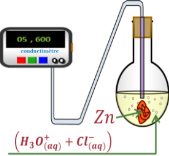
\includegraphics[width=0.16\textwidth]{./img/chimie01.png}
%%\end{center}
%\end{wrapfigure}


%\begin{wrapfigure}[1]{r}{0.5\textwidth}
	%\vspace{0.5cm}
%\begin{center}
  %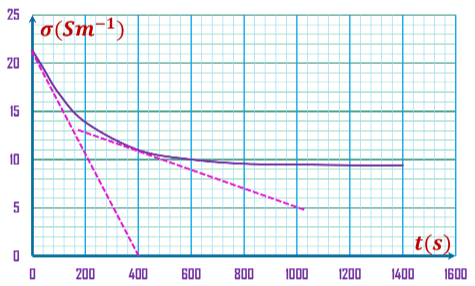
\includegraphics[width=0.5\textwidth]{./img/chimie02.png}
%\end{center}
%\end{wrapfigure}
Définition: La solubilité est la quantité maximale de solide que l'on peut dissoudre dans un
litre d'eau à une température donnée.

Masse molaire atomiques en g/mol: $M(Na) = 23,0$

Solubilité dans l'eau à 25°C de l’acide benzoïque : $s = 2,57 g/L$

\textit{L’acide benzoïque $C_6H_5COOH$ (que l’on pourra noter AH) et le benzoate de sodium
$C_6H_5COONa$ (que l’on pourra noter NaA) sont des solides conservateurs alimentaires, utilisés en
particulier dans les boissons rafraîchissantes de type soda ; ils sont respectivement désignés par le code
européen E 210 et E 211. }

 \section*{Partie 1 : Étude conductimétrique et pH-métrique d’une solution d’acide benzoïque
}

On dispose d’une solution $(S_1)$ d’acide benzoïque préparer en dissolvant $m_1 = 122 mg$ d’acide
bensoique dans $V_1 = 100,0 mL$ d’eau distillée.

	\begin{tabular}{c|l}
		0,75 & \makecell[l]{\textbf{1. }Calculer $C_1$ la concentration molaire en soluté apporté de cette solution, en déduire la \\concentration
massique la solution est-elle saturée ? justifier }\\

		0,5 & \makecell[l]{\textbf{2. }Écrire l’équation chimique symbolisant la réaction de l’acide benzoïque avec l’eau. }\\

		0,75 & \makecell[l]{\textbf{3. }Calculer le taux d’avancement de cette réaction. Conclure. }\\

		0,75 & \makecell[l]{\textbf{4. }Montrer que la constante d’équilibre $K_1$ de cette réaction peut s’écrire sous forme :\\ 
		$K_1 = \frac{(\frac{\sigma}{\lambda_a + \lambda_b})^2}{C_1 - (\frac{\sigma}{\lambda_a + \lambda_b})}$ Calculer sa valeur}
			
	\end{tabular}

5. On prépare une solution saturée d’acide benzoïque. On filtre cette solution que l’on notera par la
suite $(S_2)$ son volume $V_2 = 100,0 mL$ et sa concentration $C_a$. Le pH de cette solution est 2,96.

	\begin{tabular}{c|l}
		0,75 & \makecell[l]{\textbf{5.1. } Vérifier  que la concentration de cette solution est $C_a = 2,1.10^{-2}mol/L$}\\

		 & \makecell[l]{\textbf{5.2. }On la laisse la solution $(S_2)$ s’évaporer à 25°C, jusqu’à ce que son volume diminue de $40 \%$.\\on
		constate que le pH conserve sa valeur 2,96.\\ \textbf{Remarque : seulement le solvant (eau) qui s’évapore.} }\\

	\end{tabular}
	
	\begin{tabular}{c|l}
		0,75 & \makecell[l]{\textbf{5.2.1. }La concentration de cette solution change-t-elle ? justifier}\\

		0,75 & \makecell[l]{\textbf{5.2.2. }Justifier qu’un précipité se forme au cours de cette évaporation et calculer sa masse. }\\

	\end{tabular}


	Les conductivités molaires ioniques : $ \lambda_b= \lambda_{H_3O^+}$=$35.mS.m^2/mol$ ; $\lambda_b = \lambda_{C_6H_5COO^-}$=$3,25.mS.m^2/mol$


\section*{Partie 2 : Étude de la réaction d’acide benzoïque avec les ions éthanoate }

Dans un flacon contenant de l’eau, on introduit une quantité $n_0 = 3.10^{-3} mol$ d’acide benzoïque
et une même quantité $n_0 = 3.10^{-3} mol$ d'éthanoate de sodium $CH_3COONa$. On obtient une solution
aqueuse de volume $V=100 mL$. On modélise la transformation chimique qui s’effectue par l’équation
suivante :

$$\ce{C_6H_5COOH_{(aq)} + CH_3COOH_{(aq)} <=> C_6H_5COO^- + CH_3COOH_{(aq)}}$$

La mesure de la conductivité du milieu réactionnel à l’équilibre donne la valeur $\sigma = 255 mS. m^{-1}$
\textbf{On néglige la conductivité molaire ionique des ions $H_3O^+$ et $HO^-$}

$\lambda_1 = \lambda_{Na^+} = 5,0 mS.m^2/mol \hspace{0.5cm} \lambda_2 = \lambda_{C_6H_5COO^-}=3,25.mS.m^2/mol \hspace{0.5cm} \lambda_3 = \lambda_{CH_3COO^-}=4,1 mS.m^2/mol$

\begin{tabular}{c|l}
	1  & \makecell[l]{ \textbf{1. }Montrer que l’expression de l’avancement finale de la réaction s’écrit :
	$x_f = \frac{\sigma.V - n_0.(\lambda_1 - \lambda_3)}{\lambda_2 - \lambda_3}$
\\Calculer sa valeur.}\\

	1	& \makecell[l]{\textbf{2. }Trouver l’expression de la constante d’équilibre $K_2$ associé à l’équation de la réaction en \\fonction de $x_f$ et $n_0$. Calculer sa valeur.}\\

\end{tabular}

%\hrulefill
%\Large{Physique 13pts/78min}
%\hrulefill\\
\begin{center}
    %\vspace{.60cm}
\hrulefill
\Large{Physique 13pts - 75min}
\hrulefill\\
    \emph{Les  parties sont indépendantes}
\end{center}

%\vspace{-1cm}
\section*{Partie 1 : La radioactivité au service de la médecine\dotfill(5.5pts)}

%\begin{wrapfigure}[2]{r}{0.19\textwidth}
  %\begin{center}
	  %\vspace{-2cm}
	%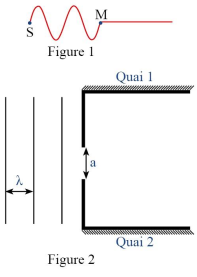
\includegraphics[width=0.19\textwidth]{./img/ex6.png}
  %\end{center}
%\end{wrapfigure}
Le noyau de sodium $_{11}^{24}Na$ se désintègre spontanément en noyau de magnésium $_{12}^{24}Mg$ avec production d’une particule X.


\begin{tabular}{c|l}

	0,5 & \makecell[l]{\textbf{1. }Identifier la particule X et préciser le type de radioactivité du sodium 24.}\\

	0,5 & \makecell[l]{\textbf{2. }Comparer la stabilité des deux noyaux $_{11}^{24}Na$ et $_{12}^{24}Mg$. }\\
	\end{tabular}

\textbf{3. }À la suite d’un accident de circulation, une personne a perdu un volume de sang. Afin de déterminer
le volume sanguin perdu, on injecte au patient à l’instant $t_0 = 0$ un volume $v_0 = 5,00mL$ d’une
solution de sodium 24 de concentration $C_0 = 1,00.10^{-3}mol/L$.

	\begin{tabular}{c|l}

		0,5 & \makecell[l]{\textbf{3.1 }Calculer la quantité de matière $n_0$ de sodium 24 injecté à l’instant $t_0 = 0$. }\\

		0,5 & \makecell[l]{\textbf{3.2 }Vérifier que l’activité de l’échantillon injecté à $t_0$ vaut $a_0 = 3,86.10^{13}Bq$ }\\

		0,5 & \makecell[l]{\textbf{3.3 }Déterminer la quantité de matière $n_1$ de sodium restant à $t_1 = 3h$. }\\
		
		0,5 & \makecell[l]{\textbf{3.4 }A l’instant $t_1 = 3h$, l’analyse d’une prise de sang du patient de volume $v_p = 2,00mL$, indique \\la
		présence de $n_p = 2,1.10^{-9} mol$ de sodium 24. En déduire le volume $V_{perdu}$ du sang perdu, en\\
considérant que l’organisme humain contient 5L du sang, et que le sodium est uniformément\\
réparti dans le sang. }\\
	\end{tabular}


\textbf{4. }On donne ci-dessous le diagramme d’énergie de la désintégration du sodium 24.
	
	\begin{tabular}{c|l}

		0,5 & \makecell[l]{\textbf{4.1 }4.1.Définir l’énergie de liaison $E_l$.}\\

		0,5 & \makecell[l]{\textbf{4.2 }Calculer, en MeV, les énergies $E_{Inter1}$ et $E_{Inter2}$.}\\

		0,5 & \makecell[l]{\textbf{4.3 }A quoi correspond le bilan énergétique $\Delta{E_2}$ ? calculer sa valeur. }\\
		
	\end{tabular}


\textbf{5. } Exprimer en fonction des masses des particules et la célérité c de la lumière dans le vide, les bilans
d’énergie $\Delta{E_1}$ et $\Delta{E_3}$ et déduire la signification physique de chaque bilan.


\textbf{6. } Calculer en joule (J) l’énergie reçue par le corps du patient injecté pendant la durée $3h$ qui s’écoule
entre l’injection et le prélèvement.
\begin{figure}[h]
\begin{center}
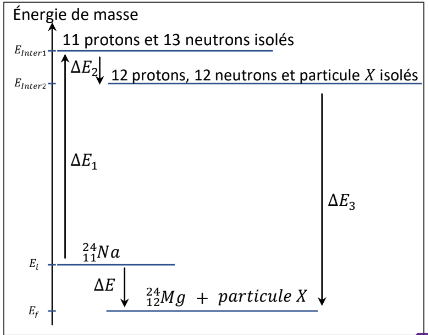
\includegraphics[width=9cm]{./diagram.png}
	\end{center}
\end{figure}
\begin{center}
\begin{tabular}{ |c|| c| c| c| c| c| }
	Particule & $_{11}^{24}Na$ & $_{12}^{24}Mg$ &  $_1^1p$ & $^1_0n$ & $^0_{-1}e$ \\ 
	Masse en u & --- & --- & 1,0072 & 1,00866 & $5,486.10^{-4}$ \\  
 Energie de liaison par
	nucléon (MeV/nucléon) & 8,062469 & 8,08907 & --- & --- & --- \\     
\end{tabular}
\end{center}



\begin{center}
\begin{tabular}{ ||c|| c|| }
	$1u = 931,4943 Mev/c^2$ & $1Mev = 1,6.10^{-13}J$ \\ 
	$t_{1/2}(_{11}^{24}Na) = 15h$ & $N_a = 6,02.10^{23} mol^{-1}$ \\  
\end{tabular}
\end{center}

\section*{Partie 2 :   La désintégration d’un isotope du bismuth\dotfill(3,5pts)}
Un isotope du bismuth $^A_ZBi$ est $\beta^{-}$ radioactif. Sa désintégration donne un noyau de polonium $^{210}_{84}Po$.
\begin{tabular}{c|l}

 0,5 & \makecell[l]{\textbf{1. } Écrire l'équation complète de désintégration nucléaire du bismuth puis représenter les deux \\noyaux père et fils
sur un digramme de Segré simplifié.}\\

 0,5 & \makecell[l]{\textbf{2. } Cette désintégration est-elle provoquée ou spontanée ? naturelle ou artificielle ? \\ordonnée ou aléatoire ?}\\

 0,5 & \makecell[l]{\textbf{3. } Quelle est l'origine de la particule $\beta^-$  émise ? Expliquer soigneusement la réponse.}\\

 0,5 & \makecell[l]{\textbf{4. } Calculer, en Mev.Nucléo$n^-1$, l'énergie de liaison par nucléon $\xi_1$ du noyau de bismuth utilisé.}\\

 0,5 & \makecell[l]{\textbf{5. } Sachant que l'énergie de liaison du noyau de polonium est $El_2 = 1539,02Mev$, comparer la \\stabilité des noyaux de $^A_ZBi$ et de  $^{210}_{84}Po$.}\\

 0,5 & \makecell[l]{\textbf{6. } Pourquoi ne peut-on pas parler de l’énergie de liaison d’un électron, d’un neutron \\ou d’un proton ?}\\
 
0,5 & \makecell[l]{\textbf{7. } Calculer, en Mev, l'énergie Elib libérée par cette réaction nucléaire en s’appuyant sur les valeurs \\des énergies de
liaison des particules présentes.}\\

 \end{tabular}

\textbf{Données :} $m(Bi) = 210,0535 u$ ; $m(n) =1,0086 u$ ; $m(p)= 1,007276 u$ ; $m (\beta^-) = 0.000549 u$ ; $m (Po) = 210,0362 u$; $1u = 1,66.10^{-27} kg$.


\section*{Partie 3 : La décroissance radioactive du bismuth\dotfill(9pts)}

A l'instant initial $t = 0$, on considère un échantillon de bismuth de masse $m_0 = 1g$. Soit m(t) la masse du bismuth
restant à la date t où t est exprimée en jours et md(t) la masse désintégrée à la même date t.

\begin{tabular}{c|l}

	1 & \makecell[l]{\textbf{1. } En appliquant la loi de décroissance radioactive, déterminer l’expression de \\m(t) en fonction de $m_0$, de la période
	radioactive $t_{1/2}$ et de t.}\\

	1 &\makecell[l]{\textbf{2. }Calculer la valeur de la période radioactive du bismuth (en jours) \\sachant que : $4.m(t+11) = m (t)$ (t en jrs). }\\ 
	1 &\makecell[l]{\textbf{3. }Quel est le pourcentage de la masse désintégrée de bismuth à la date $t = 18 jours$ ? } \\
	1 &\makecell[l]{\textbf{4. }Déterminer l'activité radioactive a0 de l'échantillon à la date t = 0 . } \\
	

\end{tabular}




\end{document}
